% A pure minimalistic LaTeX-Beamer theme for everyone to use.
% Copyright (C) 2020 Kai Norman Clasen

% This program is free software: you can redistribute it and/or modify
% it under the terms of the GNU General Public License as published by
% the Free Software Foundation, either version 3 of the License, or
% (at your option) any later version.

% This program is distributed in the hope that it will be useful,
% but WITHOUT ANY WARRANTY; without even the implied warranty of
% MERCHANTABILITY or FITNESS FOR A PARTICULAR PURPOSE.  See the
% GNU General Public License for more details.

% You should have received a copy of the GNU General Public License
% along with this program.  If not, see <https://www.gnu.org/licenses/>.

% This file is part of beamerthemepureminimalistic.

% If problems/bugs are found or enhancements are desired, please contact
% me over: https://github.com/kai-tub/latex-beamer-pure-minimalistic

\documentclass[aspectratio=169]{beamer}
% should also look nice for the classic aspectratio
% of course, than the text has to be refitted
% \documentclass{beamer}
% Will be ignored if LuaTeX engine is used
\usepackage[utf8]{inputenc}
\usepackage{tikz}
%\usetheme[darkmode, showmaxslides]{pureminimalistic}
\usetheme[lightmode, showmaxslides]{pureminimalistic}
% \renewcommand{\pageword}{}
% \renewcommand{\logoheader}{\vspace{1.5em}}
%\usepackage[backend=biber, doi=false, maxbibnames=2, maxcitenames=2,%
%            style=numeric, sorting=none, url=false, eprint=false]{biblatex}
%\addbibresource{demo_bib.bib}
\usepackage{natbib}
\bibliographystyle{apalike}

% this makes it possible to add backup slides, without counting them
\usepackage{appendixnumberbeamer}
\renewcommand{\appendixname}{\texorpdfstring{\translate{appendix}}{appendix}}

% if loaded after begin{document} a warning will appear: "pdfauthor already used"
\title[Research Background]{Research Background}
\author{Hendra Bunyamin}
% \subtitle[subtitle]{Subtitle}
\institute{Maranatha Christian University}
\date{\today}

\begin{document}
% has to be loaded outside of a frame to work!
\maketitle

% For longer table of contents, I find it cleaner to
% use no footline.
\begin{frame}[plain, noframenumbering]{Outline}
    \tableofcontents
\end{frame}

\section{Unstructured Data: Text}
\begin{frame}{Retweet Prediction }
    \begin{vfilleditems}
	\item \citet{bunyamin2016comparison} investigate the possibility of automating \textbf{retweet prediction} by utilizing machine learning models.
	\item The results show that \textbf{Random Forest} achieves the highest $F_1$ score.
	\item  Through Random Forest, the features such as \textbf{\#user listed}, \textbf{\#followers}, and \textbf{average tweets/day} determine the model's performance.
	\end{vfilleditems}
\end{frame}

\begin{frame}{Topic Clustering}
    \begin{vfilleditems}
	\item \citet{bunyamin2017automatic} explore the \textbf{application of a topic clustering model on students' final project abstracts}. 
	\item The topic clustering algorithm follows Latent Dirichlet Allocation (LDA) which is an expansion model from probabilistic latent semantic analysis (PLSA) \citep{hofmann1999probabilistic}.
	\item The results of clustering are obscure and difficult to interpret. We believe the clustering model is not suitable for this problem.
\end{vfilleditems}	
\end{frame}

\begin{frame}{Text Classification}
    \begin{vfilleditems}
	\item \citet{bunyamin2019topic}  study \textbf{text classification problem} from students' final projects. Specifically, the features are extracted from abstracts, chapter 1, chapter 2, and chapter 3.
	\item Ridge classifier, passive-aggressive,  linear Support Vector Classifier (SVC), and Stochastic Gradient Descent (SGD) classifier gain the highest accuracy among all 12 text classification models. Surprisingly, the deep learning models  are unable to attain results as comparable as the ones of linear models.
\end{vfilleditems}		
\end{frame}

\begin{frame}{Language Model $\Rightarrow$ Text Classification}
	\begin{vfilleditems}
		\item \citet{bunyamin2021utilizing}  investigates an adoption of the transfer learning technique named Universal Language Model for Fine-tuning (ULMFiT) \citep{howard-ruder-2018-universal}.
		\item  The experiments show that ULMFiT achieves high accuracy ($\approx 93\%$); additionally, this high performance can mitigate the overfitting symptom.
	\end{vfilleditems}		
\end{frame}

\section{Structured Data: Time Series}
\begin{frame}{Classical vs. Deep Learning}
	\begin{vfilleditems}
	\item \citet{Bunyamin_2021} study the utilization of classical and deep learning time series prediction models in the case of Indonesian economic growth. 
	\item The dataset comprises World Development Indicators of Indonesia from 1962 to 2016. 
	\item Through experiments, Seasonal Autoregressive Integrated Average (SARIMA) and Convolutional LSTM give the best performance based on Root-Mean-Square Error (RMSE).
\end{vfilleditems}			
\end{frame}

\section{Unstructured Data: Images}
\begin{frame}{Breast Cancer Histopathological Image Classification}
	\begin{vfilleditems}
		\item \citet{ice-tes22} implement \textbf{Progressive Resizing Approach} (PRA). The idea is very simple, that is to start training using small images and finally end the training using large images.
		\item Another highlight of the research is the use of \textbf{Vahadane technique}  \citep{vahadane2016structure} which solves both stain separation and color normalization problems.
		\item The result shows that PRA achieves a promising performance measured by $F_1$ score.
	\end{vfilleditems}			
\end{frame}

\begin{frame}{Building Damage Image Segmentation}
	\begin{vfilleditems}
	\item \citet{toba2023masking}  develop \textbf{transfer learning models} using low-cost masking pre-processing in the experimental building damage (xBD) dataset, a large-scale dataset for advancing building damage assessment.
	\item The experiments show that ResNet-34 is the best with an F1 score of 71.93\%, and an intersection over union (IoU) of 66.72\%.
\end{vfilleditems}				
\end{frame}


%\section{Aspect ratio}
%\begin{frame}[fragile]{Aspect ratio}
%    This pdf uses a 16:9 aspect ratio. To utilize
%    this version, simply use:
%    \begin{verbatim}
%    \documentclass[aspectratio=169]{beamer}
%    \end{verbatim}
%    \vfill
%    The default is a 4:3 aspect ratio.
%    \begin{verbatim}
%    \documentclass{beamer}
%  \end{verbatim}
%\end{frame}
%
%\section{vfilleditems}
%\begin{frame}{Using itemize}
%    \begin{itemize}
%        \item I like it to have my bullet points
%        \item evenly spaced from one another
%        \item then few bullet points, are not crammed on
%              the upper part of the slide
%              like it is right now with itemize
%    \end{itemize}
%\end{frame}
%
%\begin{frame}[fragile]{Using vfilleditems}
%    \begin{verbatim}
%    Use the provided \vfilleditems environment
%    to create nicely spaced bullet points.
%
%    \begin{vfilleditems}
%      \item I like it to have my bullet points
%      \item evenly spaced from one another
%      \item then few bullet points, are not crammed on
%      the upper part of the slide
%    \end{vfilleditems}
%    \end{verbatim}
%\end{frame}
%
%\begin{frame}{Using vfilleditems}
%    \begin{vfilleditems}
%        \item I like it to have my bullet points
%        \item evenly spaced from one another
%        \item then few bullet points, are not crammed on
%        the upper part of the slide
%    \end{vfilleditems}
%\end{frame}
%
%\begin{frame}{Using vfilleditems}
%    \begin{vfilleditems}
%        \item Note that the overlay specification
%        is a bit different to \emph{itemize}
%        \item For grouped overlay specifications, simply add it
%        directly after the environment:
%        \begin{vfilleditems}
%            \item \texttt{\textbackslash{}begin\{vfilleditems\}<+->}
%        \end{vfilleditems}
%    \end{vfilleditems}
%\end{frame}
%
%
%\section{Fonts}
%\begin{frame}[fragile]{Fonts}
%    Fonts:
%
%    {\small This is small}
%
%    This is normal size
%
%        {\large This is large}
%    \vfill
%    Per default the \emph{Fira Font} Package is
%    used. The \emph{Noto Font} is also bundled into this
%    package.
%\end{frame}
%
%\begin{frame}[fragile]{Fonts}
%    To use \emph{Noto} instead of \emph{Fira Fonts}
%    \begin{verbatim}
%    \usetheme[noto]{pureminimalistic}
%  \end{verbatim}
%    \vfill
%    To disable the \emph{Fira Fonts} and use the default font
%    \begin{verbatim}
%    \usetheme[customfont]{pureminimalistic}
%  \end{verbatim}
%\end{frame}
%
%\section{Color}
%\begin{frame}[fragile]{Color}
%    To overwrite the theme color
%    \begin{enumerate}
%        \item Define a new color
%        \item redefine the themes color (before document begins)
%    \end{enumerate}
%\end{frame}
%
%\begin{frame}[fragile]{Change color example}
%    \small
%    \begin{verbatim}
%  \usetheme{pureminimalistic}
%  \definecolor{textcolor}{RGB}{0, 0, 120}
%  \definecolor{title}{RGB}{0, 0, 0}
%  \definecolor{footercolor}{RGB}{133, 133, 133}
%  \definecolor{bg}{RGB}{25, 116, 210}
%
%  \renewcommand{\beamertextcolor}{textcolor}
%  \renewcommand{\beamerbgcolor}{bg}
%  \renewcommand{\beamerfootertextcolor}{footercolor}
%  \renewcommand{\beamertitlecolor}{title}
%  \end{verbatim}
%\end{frame}
%
%\begin{frame}[fragile]{Dark mode}
%    I've included a simple way to use a dark mode
%    color theme. To use the dark color mode, provide the \texttt{darkmode}
%    option.
%    \begin{verbatim}
%    \usetheme[darkmode]{pureminimalistic}
%    \end{verbatim}
%    Sometimes, the logos have to be changed to look nice on a
%    dark background. For now, I am simply loading different
%    files if \texttt{darkmode} is used.
%\end{frame}
%
%\section{Graphics}
%\begin{frame}{Logos}
%    Commands setting the logos:
%    \begin{itemize}
%        \item \texttt{\textbackslash{}logotitle} -- Command used for the title page.
%              Here \texttt{\textbackslash{}linewidth} corresponds to the entire paper width.
%        \item \texttt{\textbackslash{}logoheader} -- Command used for the header.
%              Here \texttt{\textbackslash{}linewidth} corresponds to a smaller box,
%              as the horizontal space is shared with the title.
%        \item \texttt{\textbackslash{}logofooter} -- Command used for the footer.
%              Here \texttt{\textbackslash{}linewidth} corresponds to a smaller box,
%              as the horizontal space is shared with the footer text.
%    \end{itemize}
%\end{frame}
%
%\begin{frame}[fragile]{Logos -- Load own logo}
%    To use your own logos, simply redefine the commands and adjust the sizes.
%    \begin{verbatim}
% \renewcommand{\logotitle}{\includegraphics%
%   [width=.2\linewidth]{alternative_logo/gameboy.png}}
% \renewcommand{\logoheader}{\includegraphics%
%   [width=.5\linewidth]{alternative_logo/gameboy.png}}
% \renewcommand{\logofooter}{\includegraphics%
%   [width=.15\linewidth]{alternative_logo/console.png}}
%  \end{verbatim}
%\end{frame}
%
%\begin{frame}[fragile]{Logos -- Disable logo}
%    To disable the logo, overwrite the default logo command with an empty
%    command.
%    \begin{verbatim}
% \renewcommand{\logoheader}{}
%  \end{verbatim}
%    You may want to add some vertical space if you wish to delete the \texttt{logoheader}.
%    \begin{verbatim}
% \renewcommand{\logoheader}{\vspace{1.5em}}
%  \end{verbatim}
%\end{frame}
%
%\begin{frame}{Figures}
%    I also changed the default caption settings to not
%    include \texttt{Figure:} and reduced the font size.
%    \begin{figure}[H]
%        \centering
%        \begin{columns}[T]
%            \begin{column}{.3\linewidth}
%                
\includegraphics[width=\linewidth]{example-image-a}
%                \caption{Example A}
%            \end{column}
%            \begin{column}{.3\linewidth}
%                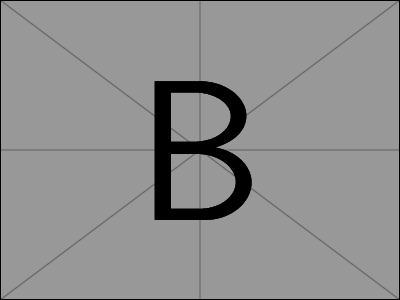
\includegraphics[width=\linewidth]{example-image-b}
%                \caption{Example B}
%            \end{column}
%        \end{columns}
%    \end{figure}
%\end{frame}
%
%\begin{frame}[fragile]{Figures -- Set background watermark}
%    There is no extra option to define a background watermark, but here
%    is a command that could be used to create one manually:
%    \vfill
%    \begin{verbatim}
%\setbeamertemplate{background}{%
%  \tikz[overlay,remember picture]%
%  \node[opacity=0.8]at (current page.center)%
%  {\includegraphics[width=.2\linewidth]%
%  {example-image-a}};%
%}
%  \end{verbatim}
%\end{frame}
%
%{
%\setbeamertemplate{background}{%
%    \tikz[overlay,remember picture]%
%    \node[opacity=0.8]at (current page.center)%
%    {\includegraphics[width=.2\linewidth]%
%        {example-image-a}};%
%}
%\begin{frame}{Figures -- Set background watermark}
%    Usually you would add this command to specific
%    frames by enclosing this command and all desired frames with
%    curly brackets.
%    \vfill
%    See the source code of this \emph{*.tex} file for an
%    example.
%\end{frame}
%}
%
%\section{Footer options}
%\begin{frame}[fragile]{Disable footer}
%    If you do not want to use a footer, disable it with:
%    \begin{verbatim}
%    \usetheme[nofooter]{pureminimalistic}
%  \end{verbatim}
%\end{frame}
%
%\begin{frame}[fragile]{Show max slide numbers}
%    For these slides, I used the option to
%    show the maximum number of slides. To activate it
%    one has to activate it with:
%    \begin{verbatim}
%    \usetheme[showmaxslides]{pureminimalistic}
%  \end{verbatim}
%    Usually, I prefer to not show the maximum number of
%    slides, as the people tend to lose focus if they know
%    the last few slides are shown.
%\end{frame}
%
%\begin{frame}[fragile]{Remove footer logo}
%    If you wish to remove the footer logo \emph{and}
%    move the page number to the right parts use:
%    \begin{verbatim}
%    \usetheme[nofooterlogo]{pureminimalistic}
%  \end{verbatim}
%\end{frame}
%
%\begin{frame}[fragile]{Change Page word}
%    If you wish to remove or change the word \emph{Page}
%    in the footer, change the value with
%    \begin{verbatim}
%    \renewcommand{\pageword}{Seite}
%  \end{verbatim}
%\end{frame}

%\section{Citations}
%\begin{frame}{Citations}
%    I've also changed the bibliography options to be minimalistic:
%
%    Just showing a simple \texttt{\textbackslash{}cite} \citep{AlexNet}
%%    \vfill
%%    \printbibliography
%\end{frame}

%\appendix % do not count the following slides for the total number
%\section*{Backup Slides}
%\begin{frame}[plain, noframenumbering]
%    \centering
%    \vfill
%    {\fontsize{40}{50}\selectfont Backup Slides}
%    \vfill
%\end{frame}
%
%\begin{frame}{What happened to the page numbering?}
%    \begin{itemize}
%        \item I've used the \texttt{appendixnumberbeamer}
%              package, which resets the frame counting after calling
%              \texttt{\textbackslash{}appendix}
%        \item Depending on the used pdf viewer, the total
%              count of frames shouldn't include the backup slides and
%              won't demotivate the audience.
%        \item Usually, I would use a \texttt{plain} frame
%              for the backup slides.
%    \end{itemize}
%\end{frame}

\section<presentation>*{\appendixname}
\subsection<presentation>*{For Further Reading}

\begin{frame}[allowframebreaks]
	\frametitle<presentation>{References}
	{\footnotesize
		%    \bibliographystyle{apalike}
		\bibliography{demo_bib}
	}    
\end{frame}

\end{document}
